\newpage
\section{Analysis}

Once the code has been completed and the functionality has been verified (See section xxx for verification) we have automated the process to run the application for every possible input size $1 \leq size \leq 128$ and collect all the timing information to conduct performance analysis and get more insight into the application's behavior under different input sizes.

Figure~\ref{fig:perf_plot} shows execution time for different valid input sizes for different configurations. To facilitate the analysis a more elaborate plot with speedups has been made in Figure~\ref{fig:speedup_plot} which shows speedups for different valid input sizes for DSP+NEON and NEON only configurations. (Note that the spikes in the plots are due to the fact that the operating system is not real-time) This figure shows us a number of useful insights:

\begin{itemize}
\item{NEON+DSP shows slowdown for $size < 60 + \epsilon$}
\item{NEON only configuration performs better for $size < 90 + \epsilon$}
\item{NEON+DSP configuration is best for $size >90 + \epsilon$}
\item{NEON only configuration performs better than serial execution $ \forall size$}

\end{itemize}

\begin{figure}[h!]
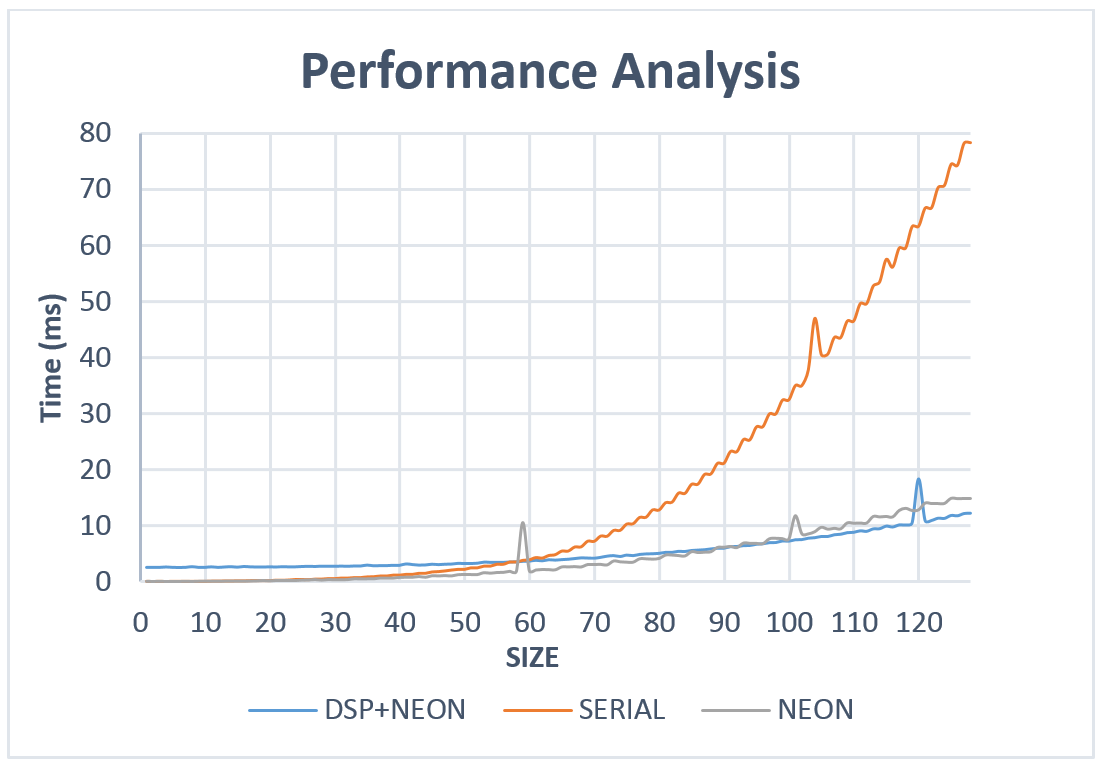
\includegraphics[width=\textwidth]{analysis/perf_plot}
\caption{Performance Analysis plot: Execution times as a function of input size for different configurations}
\label{fig:perf_plot}
\end{figure}


\begin{figure}[h!]
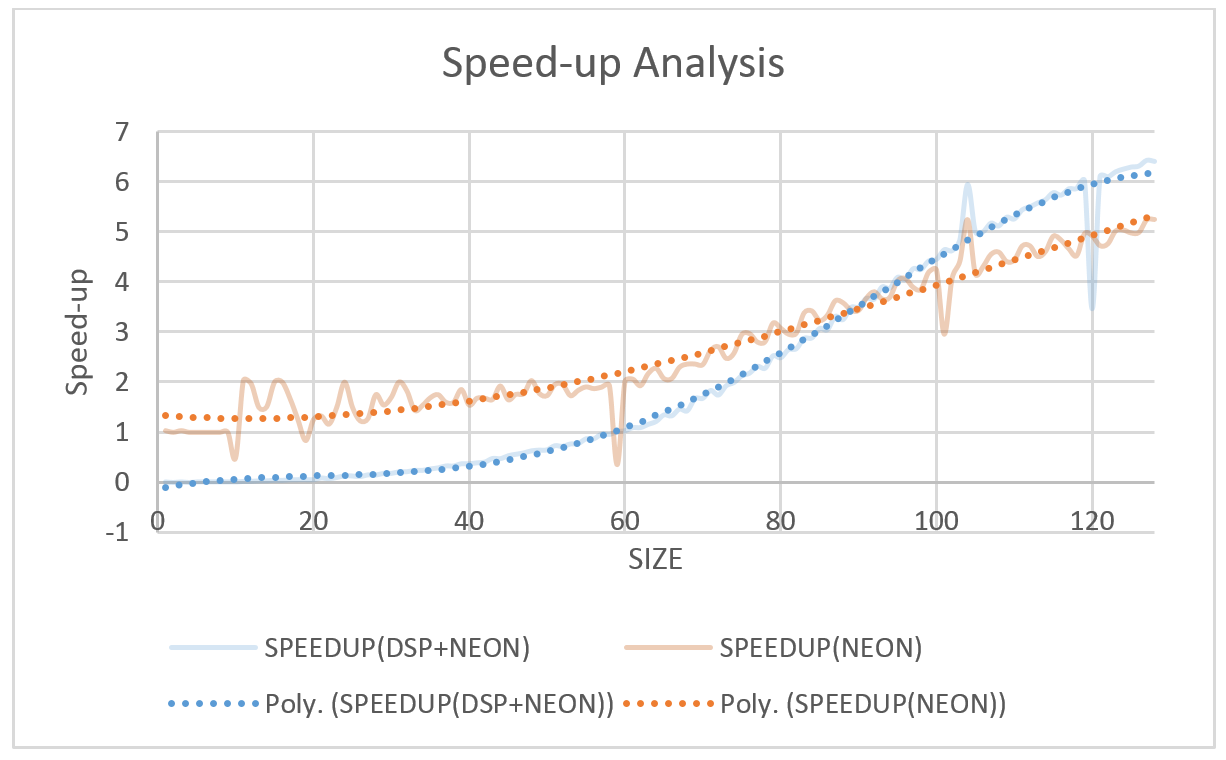
\includegraphics[width=\textwidth]{analysis/speedup_plot}
\caption{Speed-up plot: Achievable speed-up as a function of input size for different configurations}
\label{fig:speedup_plot}
\end{figure}

\subsection{Theoretical Upper Bound on the Speed-Up}
We are using the beagleboard to speed up our reference application (Multiplications). Our plan is to distribute the computational load on both the neon and DSP equally. As the DSP has two multipliers which can perform two operations simultaneously, this means that on the DSP we can perform four multiplication operations at the same time. Similarly, by using Neon we can also perform four 32 bit multiplication operations at a time. In order to simplify the calculation for the upper bound on the speed-up, we have made following assumptions:

\begin{itemize}
\item All the operations take a single clock cycle to complete.
\item The time that is consumed in communication between the processors is zero.
\item The time to load data data into the processors is negligible.
\end{itemize}

The complexity of Serial multiplications is in the order of O($n^3$). In order to make our calculations simple, we assume that $n = 16$, so our task is to perform the multiplications of two 16x16 matrices.

As serial multiplications takes $n^3$ cycles to complete in the reference implementation (since it is a triple nested for-loop over the input size), so number of cycles required to complete the multiplications for $n = 16$ would be $16^3 = 4096$. As we are distributing our work load equally on the both DSP and Neon, the effective work load for each one would be $\frac{n * n}{2}$. In our current scenario each of the processor will get $\frac{16 * 16}{2}$ matrices.

As each can perform 4 multiplication operations at a time, the time required to complete all multiplications would be $\frac{16*16}{8} = 32$. So the fraction of the reference application that is strictly serial for our platform is: $\frac{32}{4096} = 0.0078125$.

According to Amdahl's law the speed up would be $S(n) = \frac{1}{B + \frac{1 - B}{n}}$, with $n$ being the number of processors. We can regard this as being 8, as we can perform 8 calculations at the same time. Filling this in the equation gives us a theoretical upperbound on our speedup of $S(8) = \frac{1}{{0.0078125 + \frac{1 - 0.0078125}{8}}} = \frac{1}{0.1318} = 7.6$ times.
